This section reviews the dual IQC formulation for robustness analysis in the ODE setting. The results of
\textit{Robust $\mathscr{L}_2$-gain feedforward control of uncertain systems using dynamic IQCs} \cite{koserobust}
and \textit{Convex LPV synthesis of estimators and feedforwards using duality and integral quadratic constraints} \cite{venkataraman}
are the main finite-dimensional references. They will later serve as a point of comparison for the infinite-dimensional formulation based on PI operators and PIE systems.

\subsection{Köse and Scherer}
The starting point is the standard IQC robustness theorem.
\begin{theorem}[Megretski and Rantzer~\cite{megretski1997system}]
    Suppose $G$ is stable and
    \begin{enumerate}
        \item the feedback interconnection of $\tau\Delta$ and $G$ is well-defined for all $\tau \in [0,1]$;
        \item $\tau\Delta$ satisfies the IQC defined by $\Pi$ for all $\tau \in [0,1]$, i.e.,
        \begin{equation}\label{iqc}
            \ip{\bmat{q \\ \tau\Delta q}}{\Pi\bmat{q \\ \tau\Delta q}} \geq 0
            \quad \forall q \in \mathscr{L}_{2+}, \quad \forall \tau \in [0,1];
        \end{equation}
        \item $G$ satisfies
        \begin{equation}\label{primal}
            \bmat{G \\ I}^* \Pi \bmat{G \\ I} \prec 0
            \quad \text{on } \mathbb{C}_0.
        \end{equation}
    \end{enumerate}
    Then the feedback interconnection of $\Delta$ and $G$ is stable.
\end{theorem}

The dual IQC formulation used in \cite{koserobust} follows from a finite-dimensional inertia argument.
\begin{lemma}\label{lemma}
    Let $S\in\mathbb{C}^{(m+n)\times m}$ have full column rank and let
    $M = M^* \in \mathbb{C}^{(m+n)\times(m+n)}$ satisfy $\operatorname{in}(M) = (m,n,0)$
    (implying $M_{11},-M_{22}>0$). Then $S^*MS\prec 0$ if and only if
    $S_\perp^* M S_\perp \succ 0$, where $S_\perp$ forms a basis for the orthogonal
    complement of the image of $S$.
\end{lemma}

Applying Lemma~\ref{lemma} to \eqref{primal} gives the dual frequency-domain condition
\begin{equation}\label{dual}
    \bmat{G^* \\ I}^* \bmat{0 & I \\ -I & 0} \Pi^{-\top}
    \bmat{0 & I \\ -I & 0} \bmat{G^* \\ I}
    \prec 0
    \quad \text{on } \mathbb{C}_0.
\end{equation}
For later use, define the dual multiplier
\begin{equation}\label{dual_multiplier}
    \mathbf{D}(\Pi)
    := \bmat{0 & I \\ -I & 0} \Pi^{-\top} \bmat{0 & I \\ -I & 0}
    =: \Theta
    = \bmat{\Theta_{11} & \Theta_{12} \\ \Theta_{12}^* & \Theta_{22}}.
\end{equation}
Applying the same inertia argument to \eqref{iqc} yields the corresponding dual IQC
\begin{equation}\label{dual_iqc}
    \ip{\bmat{q \\ \tau\Delta^* q}}{\Theta\bmat{q \\ \tau\Delta^* q}} \leq 0
    \quad \forall q \in \mathscr{L}_{2+}, \quad \forall \tau \in [0,1].
\end{equation}

\subsection{Venkataraman and Seiler}
The duality framework in \cite{venkataraman} uses this construction together with $J$-spectral factorizations of PN multipliers.
\begin{definition}[Hu et al.~\cite{https://doi.org/10.1002/rnc.3646}]\label{PN}
    Let $\Pi=\Pi^{\sim}\in\mathbb{R}L_\infty^{(n_v+n_w)\times(n_v+n_w)}$, where
    $H^\sim(s)=H(-s)^\top$ for $H\in\mathbb{R}L_\infty$.
    Partition $\Pi$ as
    \[
        \Pi=\bmat{\Pi_{11} & \Pi_{12} \\ \Pi_{12}^{\sim} & \Pi_{22}},
    \]
    where $\Pi_{11}\in\mathbb{R}L_\infty^{n_v\times n_v}$ and
    $\Pi_{22}\in\mathbb{R}L_\infty^{n_w\times n_w}$. Then $\Pi$ is called a strict
    positive-negative (PN) multiplier if
    $\Pi_{11}(\mathrm{j}\omega)>0$ and $\Pi_{22}(\mathrm{j}\omega)<0$ for all
    $\omega\in\mathbb{R}\cup\{\infty\}$.
\end{definition}

\begin{definition}[Bart et al.~\cite{bart1979minimal} and Meinsma~\cite{meinsma1995jspectral}]\label{jfactor}
    Let
    \[
        J_{n_v,n_w}:=\bmat{I_{n_v} & 0 \\ 0 & -I_{n_w}}.
    \]
    A pair $(\hat{\Psi},J_{n_v,n_w})$ is called a $J$-spectral factorization of
    $\Pi=\Pi^{\sim}$ if
    \begin{equation}
        \Pi=\hat{\Psi}^{\sim}J_{n_v,n_w}\hat{\Psi},
        \qquad
        \hat{\Psi},\hat{\Psi}^{-1}\in
        \mathbb{R}H_\infty^{(n_v+n_w)\times(n_v+n_w)}.
    \end{equation}
\end{definition}

\begin{remark}
    The strict PN condition in Definition~\ref{PN} is a convenient class of admissible multipliers, but it is stronger than what the duality argument itself requires. The essential requirement is the existence of a stable, bistable $J$-spectral factorization in the sense of Definition~\ref{jfactor}.

    For example, an off-diagonal multiplier
    \[
        \Pi=\bmat{0 & \Pi_{12} \\ \Pi_{12}^{\sim} & 0}
    \]
    is not strict PN, but it admits a $J$-spectral factorization whenever the factor below is stable and bistable:
    \begin{equation}
        \Pi=\hat{\Psi}^{\sim}J\hat{\Psi},\qquad
        \hat{\Psi}:=\frac{1}{\sqrt{2}}\bmat{I & \Pi_{12} \\ I & -\Pi_{12}},
        \qquad
        J:=\bmat{I & 0 \\ 0 & -I}.
    \end{equation}
    More generally, consider
    \[
        \Pi=\bmat{\Pi_{11} & \Pi_{12} \\ \Pi_{12}^{\sim} & \Pi_{22}},
        \qquad
        \Pi_{22}<0,\qquad
        \Pi_{11}-\Pi_{12}\Pi_{22}^{-1}\Pi_{12}^{\sim}>0.
    \]
    Then $\Pi$ admits the $J$-spectral factorization
    \begin{equation}
        \Pi=\Psi^{\sim}J\Psi,\qquad
        \Psi:=\bmat{F_{11} & 0 \\ F_{22}\Pi_{22}^{-1}\Pi_{12}^{\sim} & F_{22}},
        \qquad
        J:=\bmat{I & 0 \\ 0 & -I},
    \end{equation}
    where
    \[
        F_{11}^{\sim}F_{11}
        =\Pi_{11}-\Pi_{12}\Pi_{22}^{-1}\Pi_{12}^{\sim},
        \qquad
        F_{22}^{\sim}F_{22}=-\Pi_{22}.
    \]
    This form includes the preceding examples after choosing the corresponding block factors.
\end{remark}

The state-space version of the result in \cite{venkataraman} can be described as follows. Suppose
$\Pi=\hat{\Psi}^{\sim}J\hat{\Psi}$ is a $J$-spectral factorization as in Definition~\ref{jfactor}. Then the dual IQC can be written in factored form as
\begin{equation}
    \ip{\mathbf{D}(\hat{\Psi})\bmat{z_\Delta \\ \tau\Delta^* z_\Delta}}
    {J\mathbf{D}(\hat{\Psi})\bmat{z_\Delta \\ \tau\Delta^* z_\Delta}}
    \leq 0
    \quad \forall z_\Delta \in \mathscr{L}_{2+}, \quad \forall \tau \in [0,1].
\end{equation}
First write the generalized plant as
\begin{equation}\label{gp_realization}
    \bmat{\dot{x}_G(t) \\ z_\Delta(t) \\ z(t)}
    =
    \bmat{
        A & B_\Delta & B_w \\
        C_\Delta & D_{\Delta} & D_{\Delta w} \\
        C_z & D_{z\Delta} & D_{zw}
    }
    \bmat{x_G(t) \\ w_\Delta(t) \\ w(t)},
\end{equation}
where $w$ and $z$ denote the exogenous input and performance output, respectively. Next, let $\hat{\Psi}\bmat{z_\Delta \\ w_\Delta}$ have the realization
\begin{equation}
    \bmat{\dot{x}_\Psi(t) \\ \tilde{z}_\Delta(t) \\ \tilde{w}_\Delta(t)}
    =
    \bmat{
        A_\Psi & B_\Psi^{z} & B_\Psi^{w} \\
        C_\Psi^z & D_\Psi^{zz} & D_\Psi^{zw} \\
        C_\Psi^w & D_\Psi^{wz} & D_\Psi^{ww}
    }
    \bmat{x_\Psi(t) \\ z_\Delta(t) \\ w_\Delta(t)}.
\end{equation}
Let $x:=\bmat{x_G \\ x_\Psi}$. Augmenting the generalized plant \eqref{gp_realization} with the multiplier realization gives
\begin{equation}\label{augmented_gp_multiplier}
    \bmat{
        \dot{x}(t) \\
        \tilde{z}_\Delta(t) \\
        \tilde{w}_\Delta(t) \\
        z(t)
    }
    =
    \bmat{
        \mcl{A} & \mcl{B}_\Delta & \mcl{B}_w \\
        \mcl{C}_{\tilde{z}} & \mcl{D}_{\tilde{z}\Delta} & \mcl{D}_{\tilde{z}w} \\
        \mcl{C}_{\tilde{w}} & \mcl{D}_{\tilde{w}\Delta} & \mcl{D}_{\tilde{w}w} \\
        \mcl{C}_z & \mcl{D}_{z\Delta} & \mcl{D}_{zw}
    }
    \bmat{
        x(t)\\
        w_\Delta(t) \\
        w(t)
    }.
\end{equation}
The calligraphic matrices in \eqref{augmented_gp_multiplier} are
\begin{align}
    \mcl{A}
    &:=
    \bmat{
        A & 0 \\
        B_\Psi^z C_\Delta & A_\Psi
    },
    &
    \mcl{B}_\Delta
    &:=
    \bmat{
        B_\Delta \\
        B_\Psi^zD_\Delta+B_\Psi^w
    },
    &
    \mcl{B}_w
    &:=
    \bmat{
        B_w \\
        B_\Psi^zD_{\Delta w}
    }, \label{augmented_state_matrices}\\
    \mcl{C}_{\tilde{z}}
    &:=
    \bmat{D_\Psi^{zz}C_\Delta & C_\Psi^z},
    &
    \mcl{D}_{\tilde{z}\Delta}
    &:=
    D_\Psi^{zz}D_\Delta+D_\Psi^{zw},
    &
    \mcl{D}_{\tilde{z}w}
    &:=
    D_\Psi^{zz}D_{\Delta w}, \nonumber\\
    \mcl{C}_{\tilde{w}}
    &:=
    \bmat{D_\Psi^{wz}C_\Delta & C_\Psi^w},
    &
    \mcl{D}_{\tilde{w}\Delta}
    &:=
    D_\Psi^{wz}D_\Delta+D_\Psi^{ww},
    &
    \mcl{D}_{\tilde{w}w}
    &:=
    D_\Psi^{wz}D_{\Delta w}, \nonumber\\
    \mcl{C}_z
    &:=
    \bmat{C_z & 0},
    &
    \mcl{D}_{z\Delta}
    &:=
    D_{z\Delta},a
    &
    \mcl{D}_{zw}
    &:=
    D_{zw}. \nonumber
\end{align}

Figure~\ref{resultvenkataraman} summarizes the primal-dual correspondence used in \cite{venkataraman}. The passage from the top-right realization to the bottom-right realization can be read in the following steps.
\begin{enumerate}
    \item Start with the primal interconnection in the top-right diagram, where the generalized plant is augmented with the $J$-spectral factor $\hat{\Psi}$ as in \eqref{augmented_gp_multiplier}. This realization gives the primal dissipation inequality and the corresponding LMI.

    \item One can then apply a congruence transformation on the LMI of the form
    \begin{equation}
        T =
        \bmat{
            I & 0 & 0 \\
            -\mcl{D}^{-1}_{\tilde{w}w}\mcl{C}_{\tilde{w}} & \mcl{D}^{-1}_{\tilde{w}w} & -\frac{1}{\sqrt{\gamma}}\mcl{D}^{-1}_{\tilde{w}w}\mcl{D}_{\tilde{w}z} \\
            0 & 0 & \frac{1}{\sqrt{\gamma}}I
        }.
    \end{equation}
    This gives the system on the top-left diagram and shows equivalent LMI conditions. The factor $\gamma$ is included in \cite{venkataraman}, but is not essential to the duality argument itself. Avoiding this scaling leaves the framework open to other performance descriptions, such as passivity, $H_\infty$ performance, and quadratic performance. 
    \item The top-left realization is the same augmented plant--multiplier
    interconnection after the algebraic loop has been closed by this
    substitution. In realization coordinates, this can be interpreted as a
    variable reorganization of the spectral factor, but the LMI step only uses
    the congruence.

    \item Apply Lemma~\ref{lemma} to the top-left primal system. This produces the dual realization shown in the bottom-left diagram.

    \item After applying the inverse congruence on the dual side, the
    bottom-right system is LMI-equivalent to the bottom-left system. In this
    final form the scaled signals represent an input-output mapping, which is
    the representation used for synthesis in \cite{venkataraman}.
\end{enumerate}

\begin{figure}[ht]
    \centering
    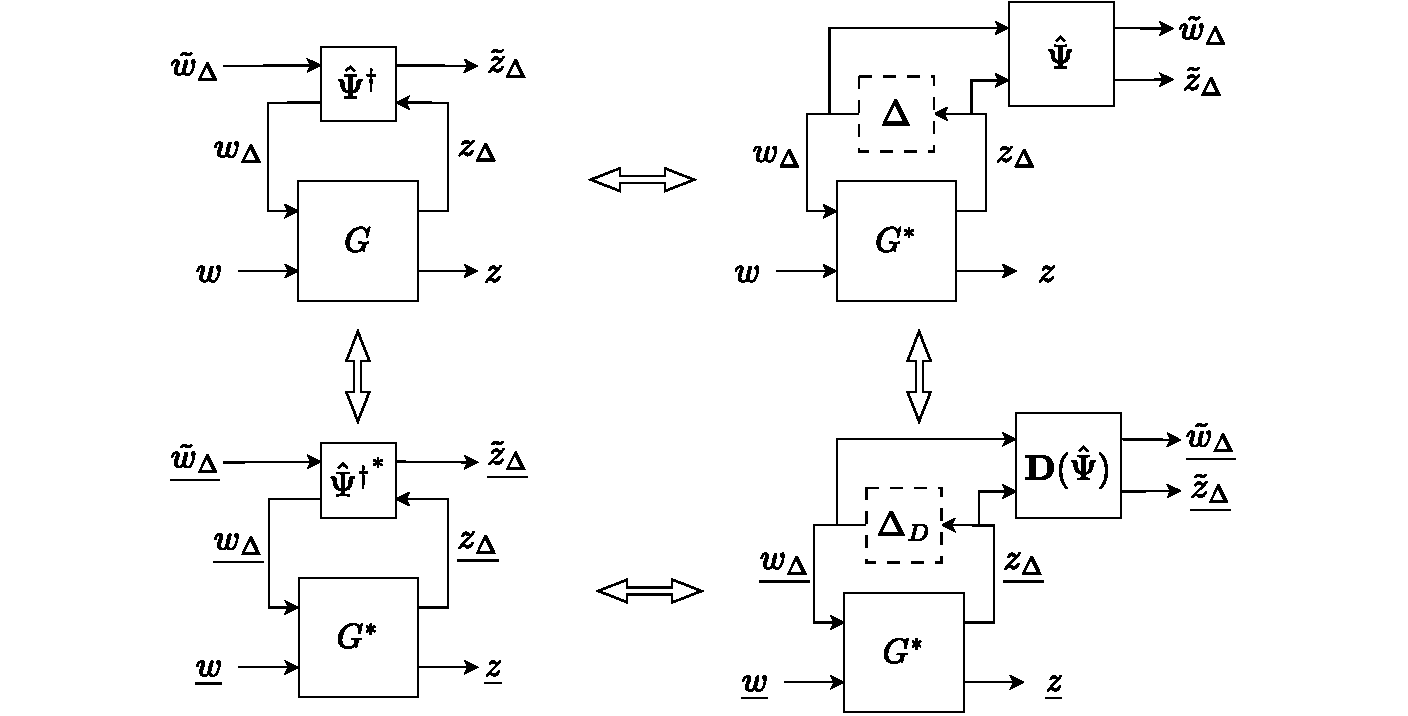
\includegraphics[width=0.8\textwidth]{Figures/Venkataraman.pdf}
    \caption{Primal-dual correspondence in \cite{venkataraman}. Venkataraman and Seiler include an $\alpha$-scaling of the multiplier. In their notation $\alpha=\sqrt{\gamma}$; here this scaling is avoided by using a different congruence transformation.}
    \label{resultvenkataraman}
\end{figure}
